\documentclass[11pt]{article}
\usepackage[margin=1in]{geometry}
\usepackage{amsmath,amssymb}
\usepackage{booktabs,tabularx,array,longtable}
\usepackage{enumitem}
\usepackage{xcolor}
\usepackage[hidelinks]{hyperref}
\usepackage{titlesec}
\usepackage{fancyhdr}
\usepackage{microtype}
\usepackage{lmodern}
\usepackage[T1]{fontenc}
\usepackage{float}
\usepackage{graphicx}
\usepackage{caption}
\usepackage[most]{tcolorbox}
\usepackage{adjustbox}
\usepackage[htt]{hyphenat}
\sloppy

\definecolor{jhublue}{RGB}{0,45,114}
\definecolor{boxgray}{RGB}{244,246,250}
\titleformat{\section}{\large\bfseries\color{jhublue}}{\thesection}{0.6em}{}
\titleformat{\subsection}{\normalsize\bfseries}{\thesubsection}{0.6em}{}
\titleformat{\subsubsection}{\normalsize\itshape}{\thesubsubsection}{0.6em}{}
\setlist{itemsep=2pt,topsep=3pt}
\captionsetup{font=small,labelfont=bf}
\pagestyle{fancy}\fancyhf{}
\cfoot{\small\thepage}
\renewcommand{\headrulewidth}{0.3pt}
\emergencystretch=3em

\newcommand{\PSI}{\mathrm{PSI}}
\newcommand{\file}[1]{\texttt{\small #1}}
\newtcolorbox{summarybox}{colback=boxgray,colframe=jhublue,boxrule=0.6pt,arc=2pt,left=6pt,right=6pt,top=4pt,bottom=4pt,fonttitle=\bfseries,title=Summary}
\newtcolorbox{conceptbox}[1]{colback=white,colframe=jhublue!60,boxrule=0.4pt,arc=2pt,left=6pt,right=6pt,top=3pt,bottom=3pt,fonttitle=\bfseries\small,title={Concept: #1}}
\newtcolorbox{whybox}{colback=boxgray,colframe=gray!50,boxrule=0.4pt,arc=2pt,left=6pt,right=6pt,top=3pt,bottom=3pt}

\usepackage{subcaption}
\usepackage{listings}
\lstdefinelanguage{Stata}{
  morekeywords={use,merge,keep,drop,gen,replace,egen,reghdfe,ivreghdfe,psmatch2,
    csdid,did_imputation,eventstudyinteract,foreach,forvalues,if,else,program,define,
    end,args,scalar,return,local,global,sensemakr,test,estat,bysort,collapse,save,
    capture,noisily,post,postfile,postclose,preserve,restore,count,summarize,do,
    import,delimited,list,format,xtset,winsor2,absorb,cluster},
  sensitive=true,
  morecomment=[l]{*},
  morecomment=[l]{//},
  morestring=[b]"
}
\lstset{language=Stata,basicstyle=\ttfamily\scriptsize,keywordstyle=\color{jhublue}\bfseries,
  commentstyle=\color{gray}\itshape,stringstyle=\color{teal!70!black},
  frame=single,rulecolor=\color{gray!40},backgroundcolor=\color{boxgray},
  breaklines=true,breakatwhitespace=false,columns=fullflexible,keepspaces=true,
  xleftmargin=4pt,xrightmargin=4pt,aboveskip=6pt,belowskip=6pt,
  showstringspaces=false,literate={-}{-}1}
\newcommand{\shot}[2]{\begin{figure}[H]\centering\includegraphics[width=#2\linewidth]{shots/#1}\end{figure}}
\lhead{\small Replication of Zhang et al.\ (2026): Tasks 1--3}
\rhead{\small Sahil, Johns Hopkins University}

\begin{document}

\begin{center}
{\LARGE\bfseries Replication of ``China's Solar Expansion Policy\\[2pt] Reduces Bird Diversity''}\\[6pt]
{\large Report on Tasks 1--3: methods, Stata code, results and screenshots}\\[6pt]
{\small Zhang et al.\ (2026), \textit{Science} 393, 831}\\[2pt]
{\small Prepared by Sahil, Research Assistant to Prof.\ Paul J.\ Ferraro, Johns Hopkins University \quad$\cdot$\quad November 2026}\\[2pt]
{\small All analysis done in Stata (StataNow/BE 19.5). Project folder: \file{Solar\_Birds\_Replication/}}
\end{center}

\begin{summarybox}
\small
\textbf{The paper says:} counties with more solar policy have lower bird diversity (main effect $-0.0125$).\\[3pt]
\textbf{Task 1 (Reproduce).} All 12 published numbers we checked reproduce exactly from the authors' code and data. But most places counted as ``no solar policy'' are cities whose policy data is \emph{missing}. Comparing like with like (urban $\times$ month effects) shrinks the effect to $-0.0027$ ($p=0.47$). The instrument fails a validity test, and the matching weights were never applied.\\[3pt]
\textbf{Task 2 (Sensitivity).} A hidden factor explaining only about 2\% of the leftover variation would erase the result (about 1\% would make it insignificant). The city-vs-countryside trend is far stronger than that.\\[3pt]
\textbf{Task 3 (Staggered DiD).} Following counties before and after their first solar policy, four estimators find \emph{no decline} in bird diversity.\\[3pt]
\textbf{Conclusion:} the study's data do not show that solar policy harms birds.
\end{summarybox}

\tableofcontents
\newpage

%==========================================================================
\section*{How the project is organised}
\addcontentsline{toc}{section}{How the project is organised}
\begin{table}[H]\centering\small
\begin{tabularx}{\linewidth}{l>{\raggedright\arraybackslash}X}
\toprule
\file{run\_all.do} & Runs every task from start to finish\\
\file{00\_config.do} & Folder paths, the list of control variables, package installation\\
\file{00\_Original\_Package/} & Untouched copy of the authors' code and 46 data files\\
\file{01\_Task1\_Replication/} & Task 1: code \file{1\_1}--\file{1\_6}, data, tables, logs, report\\
\file{02\_Task2\_Sensitivity/} & Task 2: code \file{2\_1}, tables, figures, logs, report\\
\file{03\_Task3\_Staggered\_DiD/} & Task 3: code \file{3\_1}--\file{3\_5}, data, tables, figures, logs, report\\
\file{04\_Synthesis\_Report/} & This report; \file{show\_results/} holds the short do-files used for the screenshots\\
\bottomrule
\end{tabularx}
\end{table}

\begin{lstlisting}
* 00_config.do (key lines)
global ROOT   "/Users/sahiljangra/Desktop/Johns Hopkins/RA/Solar_Birds_Replication"
global DATA   "$ROOT/00_Original_Package/DATA"
global SAMPLE "$ROOT/01_Task1_Replication/data/analysis_sample.dta"
global control     "Temp Wind Pop Duration Carbon Water Green Farm Grass"
global control_noD "Temp Wind Pop Carbon Water Green Farm Grass"
foreach p in reghdfe ivreghdfe psmatch2 sensemakr csdid did_imputation eventstudyinteract {
    capture which `p'
    if _rc ssc install `p', replace
}
\end{lstlisting}

%==========================================================================
\section{Task 1: Reproduce original results using author code and data}

\subsection*{What we did}
We ran the authors' own Stata code (\file{CODE.do}) on their own data, changing only the folder paths. Then we compared 12 published numbers (Tables 1, 2, S7, S11, S12) with our output.

\subsection*{Stata code (\file{1\_4\_reproduction\_check.do}, key lines)}
\begin{lstlisting}
use "$SAMPLE", clear
* Table 1, column 3 (main result)
reghdfe ShannonBD PI $control, absorb(county year) cluster(county)
* Table S7: IV first and second stage
reghdfe   PI Sun_ccpu $control,                absorb(county year) cluster(county) keepsingleton
ivreghdfe ShannonBD (PI = Sun_ccpu) $control,  absorb(county year) cluster(county) keepsingleton
* Table S11: matching (authors' implementation)
gen treated = (PI > 0)
psmatch2 treated $control i.year, outcome(ShannonBD) neighbor(1) caliper(0.05) common
reghdfe ShannonBD PI $control if _weight != ., absorb(county year) cluster(county)
* ... each result is posted next to the paper's value; match = same to 4 decimals
\end{lstlisting}

\subsection*{Stata output}
\shot{c_s0.jpg}{0.78}
\vspace{-6pt}
\begin{whybox}\small
\textbf{Result.} \file{match = 1} in every row and \file{count if match==0} returns \textbf{0}. All 12 numbers reproduce exactly, so the authors made no calculation errors. Any problem must lie in the \emph{design}.
\end{whybox}

\shot{c_s1.jpg}{0.9}
\vspace{-6pt}
\begin{whybox}\small
\textbf{Main result, run live.} PSI coefficient $=-0.0125283$, SE $0.0036551$, $p=0.001$, $N=46{,}371$ (157 singletons dropped), 2,344 county clusters. This is exactly the paper's Table 1, column 3.
\end{whybox}

%--------------------------------------------------------------------------
\subsection{Work to understand the data structure and code}

\subsubsection*{How the dataset is built (\file{1\_2\_build\_analysis\_sample.do})}
The authors never saved a final dataset. Their code builds it each time by merging 46 small files onto the bird file. We run their preparation code unchanged, then add a few flags of our own.
\begin{lstlisting}
* Part A: authors' code (unchanged), e.g.
use "Bird.dta", clear                                   // one row = county x month
merge m:1 id YEAR using "PI.dta", keepus(PI)            // treatment (yearly)
drop if _merge==2
...
replace PI = 0 if missing(PI)                           // <-- missing policy coded as 0
drop if missing(Temp, Wind, PD, BTN, CO2, Water, Green, Farm, Grass)
gen Duration = ln(BTN+1)                                // birdwatching effort
winsor2 `var', cuts(1 99) replace                       // trim extreme values
gen Sun_ccpu = ln(sun) / CCPU                           // instrument

* Part B: our flags
merge m:1 id using `pif', keep(master match) nogen      // in_PI_file = 1 if PSI really observed
replace in_PI_file = 0 if missing(in_PI_file)
gen byte urban = mod(id,100) <= 20                      // admin code 01-20 = urban district
gen byte name_is_district = ustrregexm(<county name>, "<qu>$")  // name ends in "qu" (district)
\end{lstlisting}

\subsubsection*{What the data look like (\file{1\_3\_data\_structure.do})}
\begin{table}[H]\centering\small
\begin{tabularx}{\linewidth}{>{\raggedright\arraybackslash}Xr}
\toprule
Fact & Value\\
\midrule
Unit of observation & one county in one month\\
Rows in the analysis sample / counties & 46,528 / 2,501\\
Rows used in regressions (singletons dropped) / counties & 46,371 / 2,344\\
Months observed per county (median) & 11\\
Bird records grow from (2014) to (2023) & 563 $\to$ 13,734 county-months\\
Outcome: Shannon index, mean (SD) & 2.45 (0.98)\\
Treatment: PSI, mean (SD), max & 2.66 (4.12), 15.5\\
Share of county-months with PSI $=0$ & 59\% (median PSI is 0 every year)\\
County-years where PSI \emph{falls} (it is a yearly flow) & 12.6\%\\
Correlation of PSI with actual solar-farm area & 0.07\\
\textbf{Counties missing from the PSI file (PSI set to 0)} & \textbf{724 (43.8\% of rows)}\\
\textbf{PSI imputed as 0: urban vs rural rows} & \textbf{83.0\% vs 1.2\%}\\
\bottomrule
\end{tabularx}
\end{table}
\begin{whybox}\small
\textbf{Key point.} Most ``no-policy'' observations are \emph{cities with missing policy data}, not places that truly had no solar policy. Every later check comes back to this.
\end{whybox}

%--------------------------------------------------------------------------
\subsection{Clarify the causal estimands (the target treatment effect)}
\begin{itemize}
\item \textbf{What the paper wants:} the effect of one more unit of solar-policy stringency (PSI) on a county's bird diversity in the same month. This is an \emph{average causal response} to a continuous dose.
\item \textbf{What TWFE actually estimates:} with county and year-month fixed effects and a continuous, on-and-off treatment, $\hat\beta$ is a \emph{variance-weighted average} of many county-by-period comparisons. Some weights can be negative, and some comparisons use already-treated counties as controls. It equals a clean average effect only if effects are the same everywhere and parallel trends hold for every dose path.
\item \textbf{IV estimand:} a weighted average effect for the counties whose PSI responds to the instrument (``compliers''), assuming exclusion and monotonicity.
\item \textbf{PSM ``ATT'':} the paper calls these ATTs, but they are TWFE coefficients on a matched subsample, not matching estimates of the ATT.
\item \textbf{In one sentence:} $\hat\beta = -0.0125$ is a weighted average change in \emph{recorded} bird diversity per extra unit of \emph{newly issued} solar policy documents. It is not the effect of solar panels.
\end{itemize}

%--------------------------------------------------------------------------
\subsection{Clarify the identification strategies (TWFE, IV, others)}

\begin{table}[H]\centering\small
\begin{tabularx}{\linewidth}{l>{\raggedright\arraybackslash}X>{\raggedright\arraybackslash}X}
\toprule
Strategy & Logic & Key assumption\\
\midrule
TWFE & Compare changes in policy with changes in birds within the same county; county FE remove fixed traits, year-month FE remove common shocks & Parallel trends: without the policy, high- and low-PSI counties would have had the same bird trend\\
IV (2SLS) & Instrument $Z=\ln(\text{sunshine 1984--2013})/\text{city CPU}$ pushes PSI up & Relevance, plus \textbf{exclusion}: $Z$ affects birds only through PSI\\
PSM & Match counties with PSI$>0$ to similar ones with PSI$=0$ on observed controls & No hidden differences after matching\\
\bottomrule
\end{tabularx}
\end{table}

\subsubsection*{Check 1: is the TWFE comparison fair? (\file{1\_5\_twfe\_diagnostics.do})}
\begin{lstlisting}
reghdfe ShannonBD PI $control,                  absorb(county year)       cluster(county)  // paper
reghdfe ShannonBD PI $control if in_PI_file==1, absorb(county year)       cluster(county)  // real PSI only
reghdfe ShannonBD PI $control if urban==0,      absorb(county year)       cluster(county)  // rural only
reghdfe ShannonBD PI $control if urban==1,      absorb(county year)       cluster(county)  // urban only
reghdfe ShannonBD PI $control,                  absorb(county year#urban) cluster(county)  // urban x month FE
reghdfe ShannonBD PI $control,                  absorb(county year#prov)  cluster(county)  // province x month FE
\end{lstlisting}
\shot{c_s2.jpg}{0.9}
\vspace{-6pt}
\begin{table}[H]\centering\small
\caption{The main effect when we compare like with like}
\begin{tabularx}{\linewidth}{>{\raggedright\arraybackslash}Xcc}
\toprule
Comparison & Effect & $p$\\
\midrule
Paper (missing PSI $=0$) & $-0.0125$ & 0.001\\
Only counties with real PSI data & $-0.0027$ & 0.49\\
Rural counties only & $-0.0056$ & 0.19\\
Urban districts only & $+0.0056$ & 0.48\\
\textbf{Urban $\times$ year-month FE (screenshot above)} & $\mathbf{-0.0027}$ & \textbf{0.47}\\
Province $\times$ year-month FE & $-0.0146$ & 0.002\\
\bottomrule
\end{tabularx}
\end{table}
\begin{whybox}\small
\textbf{How to read it.} Once cities and countryside get their own monthly trends, about 80\% of the effect disappears and the rest could be chance ($p=0.47$). Province trends do not remove it, so the problem is specifically \textbf{city vs countryside}. Other checks: with the cumulative PSI stock the effect is $-0.0012$ ($p=0.58$). With the matching weights applied properly, the three PSM estimates become $-0.0051$, $-0.0052$ and $-0.0054$, none significant.
\end{whybox}

\subsubsection*{Check 2: the IV exclusion restriction (\file{1\_6\_iv\_exclusion\_tests.do})}
\paragraph{Logic of exclusion.} Sunnier places suit solar better, and when city climate-policy uncertainty (CPU) is low, governments commit more. Both raise PSI. The authors argue that long-run sunshine and city-level news uncertainty affect today's birds \emph{only} through solar policy.

\paragraph{Possible violations.}
\begin{itemize}
\item \textbf{Climate and habitat:} sunshine shapes vegetation and bird communities directly.
\item \textbf{Observer behaviour:} more sun means more birdwatching, which raises recorded diversity.
\item \textbf{Other policies:} CPU moves with \emph{all} climate policy (afforestation, inspections, coal closures, wind), which can affect birds.
\item \textbf{Economic and urban change:} CPU co-moves with construction, lighting and growth.
\item \textbf{Solar policy without solar land:} PSI barely tracks PV area, so ``through PSI'' is hard to separate from a general climate-policy channel.
\end{itemize}

\paragraph{Test (zero-first-stage, van Kippersluis and Rietveld 2018).} In counties with missing PSI, the instrument \emph{cannot} move PSI. If exclusion holds, it should then have no effect on birds.
\begin{lstlisting}
reghdfe ShannonBD Sun_ccpu $control,                  absorb(county year) cluster(county) // reduced form
reghdfe ShannonBD Sun_ccpu $control if in_PI_file==0, absorb(county year) cluster(county) // first stage = 0 here
ivreghdfe ShannonBD (PI = Sun_ccpu) $control, absorb(county year) cluster(city) keepsingleton
\end{lstlisting}
\shot{c_s3.jpg}{0.9}
\vspace{-6pt}
\begin{whybox}\small
\textbf{How to read it.} Where the instrument cannot work through PSI, it still predicts lower bird diversity: \file{Sun\_ccpu} $=-0.0021$, SE 0.0011, $p=0.048$. That is two-thirds of the full-sample reduced form ($-0.0032$), which is evidence of a direct path, so exclusion is likely violated (strong evidence, not proof, since $p$ is close to 0.05). The instrument also predicts birdwatching effort ($-0.0020$) and the CEI inspection policy ($+0.0021$). With city clustering (the level at which CPU varies), the first-stage F falls from 30.2 to 10.8. The IV estimate ($-0.126$) is ten times the TWFE estimate.
\end{whybox}

%==========================================================================
\section{Task 2: Sensitivity analysis to hidden bias (Cinelli and Hazlett, 2020)}

\subsection*{The idea in plain words}
We can never measure every confounder. So instead of asking ``is there one?'', we ask \textbf{``how strong would a hidden factor have to be to wipe out the result?''} A hidden factor's strength is measured by its partial $R^2$: how much of the \emph{leftover} variation in PSI (x-axis) and in bird diversity (y-axis) it explains, after the fixed effects and controls.

\begin{conceptbox}{the key statistics}
\begin{itemize}[leftmargin=12pt]
\item $R^2_{Y\sim D|X}$: how much of the leftover bird variation PSI explains.
\item \textbf{Robustness value $RV$}: a confounder explaining $RV$ of the leftover variation of \emph{both} PSI and birds would bring the estimate to zero.
\item \textbf{$RV_\alpha$}: the strength needed to make the estimate statistically insignificant.
\item \textbf{Benchmark bounds}: the adjusted estimate if the hidden factor were $k$ times as strong as an observed control.
\end{itemize}
\end{conceptbox}

\subsection*{Stata code (\file{2\_1\_sensitivity\_analysis.do}, key lines)}
\begin{lstlisting}
* Robustness values from t and degrees of freedom (Cinelli-Hazlett eqs 18-20; simplified for display)
program define ch_rv, rclass
    args t df q alpha lambda
    scalar f   = abs(`t')/sqrt(`df')                       // partial Cohen's f
    scalar fq  = `q'*f
    scalar rv  = 0.5*(sqrt(fq^4 + 4*fq^2) - fq^2)           // RV
    scalar fcrit = `lambda'*abs(invttail(`df'-1,`alpha'/2))/sqrt(`df'-1)
    scalar fqa = fq - fcrit
    scalar rva = cond(fqa<=0, 0, 0.5*(sqrt(fqa^4 + 4*fqa^2) - fqa^2))  // RV_alpha
    return scalar r2yd = `t'^2/(`t'^2 + `df')
end

reghdfe ShannonBD PI $control, absorb(county year) vce(unadjusted)
ch_rv t df 1 0.05                     // classical
ch_rv t df 1 0.05 lambda              // clustered: lambda = SE_cluster / SE_classical
* benchmark bounds: confounder k times as strong as each control (k = 1,2,3)
foreach b in $control {
    foreach k in 1 2 3 {
        ch_bound r2d_`b' r2y_`b' `k' `k' est se df
    }
}
* group benchmark: urban x year-month trends (partial R2 they add)
reghdfe PI $control, absorb(county year#urban) vce(unadjusted)
* cross-check with the official package on FE-demeaned data
sensemakr r_ShannonBD r_PI r_Temp ... r_Grass, treat(r_PI) benchmark(r_Duration) kd(1 2 3)
\end{lstlisting}

\subsection*{Stata output}
\shot{c_s4.jpg}{0.8}
\vspace{-6pt}
\begin{whybox}\small
\textbf{How to read it.}
\begin{itemize}[leftmargin=12pt]
\item \textbf{First table:} for the paper's model (S1), $R^2_{Y\sim D|X}=0.0005$ (PSI explains only 0.05\% of leftover bird variation), $RV=0.0216$ (2.2\%), $RV_\alpha=0.0124$ (1.2\%), and \textbf{0.93\%} with clustered SEs. For S2 (urban $\times$ month FE), the estimate is already insignificant ($RV_\alpha=0$).
\item \textbf{Second table:} a confounder twice as strong as birdwatching effort gives $-0.0067$ (clustered $t=-1.92$, not significant). Half as strong as the urban trend gives $-0.0027$ ($t=-0.72$). As strong as the urban trend flips the sign ($+0.0081$).
\end{itemize}
\end{whybox}

\subsection*{Graph 1: what happens to the estimate}
\begin{figure}[H]\centering
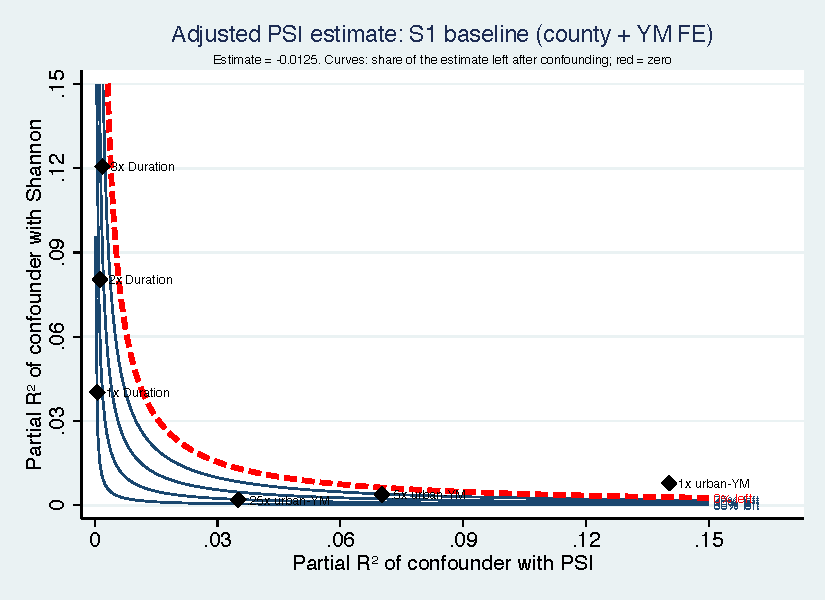
\includegraphics[width=0.74\linewidth]{fig/2_1_contour_estimate_S1.pdf}
\caption{Adjusted PSI estimate for hidden factors of different strengths (paper's model).}
\end{figure}
\begin{whybox}\small
\textbf{How to read Graph 1.} The bottom-left corner is the paper's $-0.0125$ (no hidden factor). The blue curves show how much of the effect is left (80\%, 60\%, \dots). The \textbf{red dashed curve} is where the effect reaches \textbf{zero}. ``Duration'' diamonds sit high but near the left edge, because effort explains a lot about birds but almost nothing about policy. ``Urban-YM'' diamonds sit far right, because the urban trend explains 12.3\% of PSI. The red curve hugs the axes, so a weak factor is enough, and ``1$\times$ urban-YM'' lies \emph{beyond} it (the sign flips).
\end{whybox}

\subsection*{Graph 2: when does the effect stop being significant?}
\begin{figure}[H]\centering
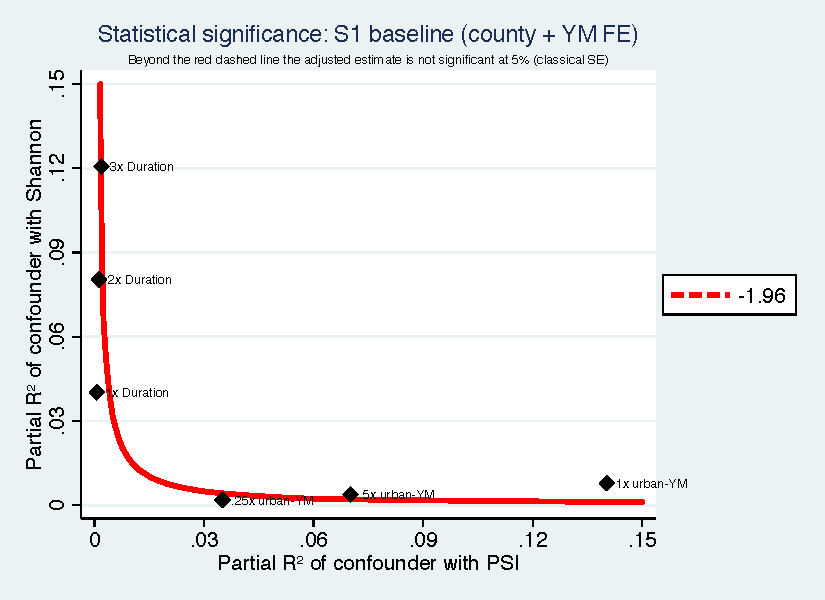
\includegraphics[width=0.74\linewidth]{fig/2_1_contour_tvalue_S1.pdf}
\caption{Where the adjusted estimate stops being significant at 5\% (paper's model).}
\end{figure}
\begin{whybox}\small
\textbf{How to read Graph 2.} Beyond the red line the result could be chance. All three urban-YM diamonds are beyond it. For birdwatching effort, $2\times$ is borderline and $3\times$ is clearly not significant.
\end{whybox}

\subsection*{Graph 3: after adding the urban trend}
\begin{figure}[H]\centering
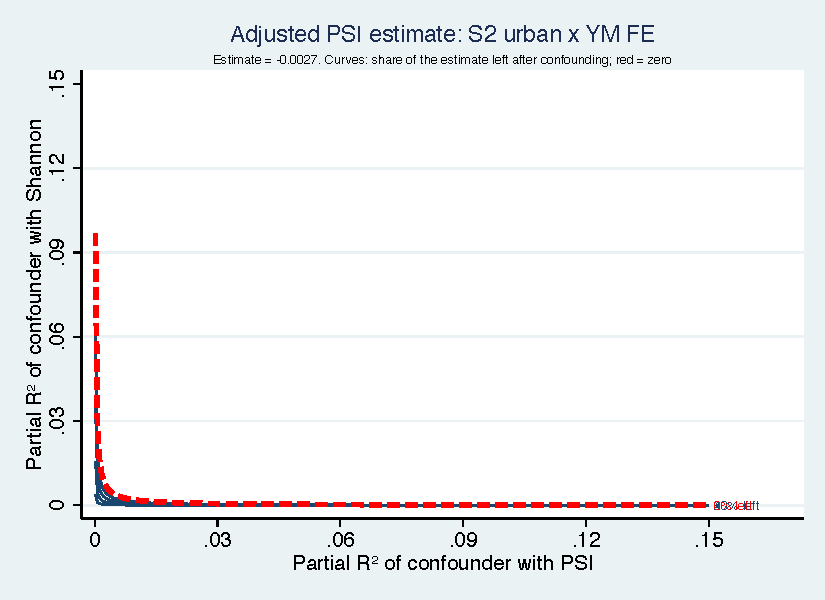
\includegraphics[width=0.66\linewidth]{fig/2_1_contour_estimate_S2.pdf}
\caption{Same graph with urban $\times$ year-month fixed effects.}
\end{figure}
\begin{whybox}\small
\textbf{How to read Graph 3.} The estimate starts at $-0.0027$, and the zero curve is pressed against the axes. Almost any hidden factor removes it.
\end{whybox}

\subsection*{Task 2 result}
The TWFE result is \textbf{fragile}. A confounder explaining about 1--2\% of residual variation overturns it, and the city-vs-countryside trend, which we can observe, is far stronger than that.

%==========================================================================
\section{Task 3: Staggered Difference-in-Differences (Baker et al., JEL)}

\subsection*{Why this matters}
Counties started solar policy in different years (2015--2023). With staggered timing and effects that may change over time, plain TWFE uses already-treated counties as controls (``forbidden comparisons'') and can be biased. Modern estimators compare each group of counties only with clean controls (never or not-yet treated).

\subsection*{Design}
\begin{itemize}
\item \textbf{Treatment:} the first year a county has PSI $>0$ (treated from then on).
\item \textbf{Main sample:} counties with real PSI data. Counties treated already in 2014 are dropped (no pre-period).
\item \textbf{Groups:} never 120; 2015: 299; 2016: 85; 2017: 75; 2018: 14; 2019: 68; 2020: 2; 2021: 91; 2022: 30; 2023: 155.
\item \textbf{Paper-style sample:} also counts the 724 missing-PSI counties as ``never treated'', as the paper implicitly does.
\end{itemize}

\subsection*{Stata code (key lines from \file{3\_1}--\file{3\_5})}
\begin{lstlisting}
* 3_1 adoption year from the full policy file
use "$DATA/PI.dta", clear
bysort id: egen first_pos = min(cond(PI > 0, YEAR, .))
gen g_main  = cond(in_PI_file==1, cond(missing(first_pos), 0, first_pos), .)
gen g_paper = cond(in_PI_file==1, g_main, 0)           // missing PSI = never treated
drop if first_pos == 2014                               // no pre-period

* 3_2 conventional TWFE event study (benchmark)
reghdfe ShannonBD lead5 lead4 lead3 lead2 lag0-lag5 $control, absorb(county year) cluster(county)

* 3_3 Callaway-Sant'Anna, not-yet-treated controls, county-year panel
csdid shannon_sa, ivar(county) time(YEAR) gvar(g_main) notyet bal(pair) rseed(20261107)
estat simple, post dropmissing
estat event, window(-5 5) post dropmissing

* 3_4 Borusyak-Jaravel-Spiess imputation, monthly data
did_imputation ShannonBD county YEAR Ei, fe(county YEAR) cluster(county) ///
    horizons(0/5) pretrends(5) autosample

* 3_5 Sun-Abraham, never-treated as the control cohort
eventstudyinteract ShannonBD `leads' `lags', cohort(cohort) control_cohort(never_main) ///
    absorb(county year) vce(cluster county)
\end{lstlisting}

\subsection*{Stata output}
\begin{figure}[H]\centering
\begin{subfigure}{0.49\linewidth}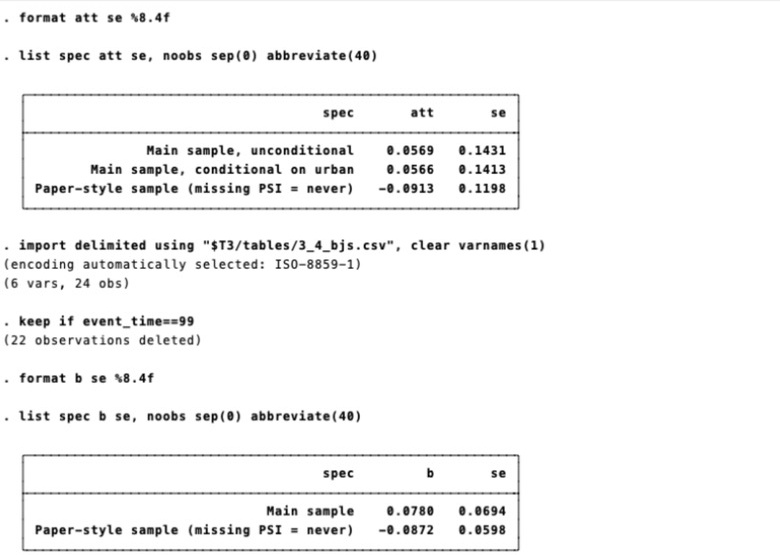
\includegraphics[width=\linewidth]{shots/c_s5a.jpg}\end{subfigure}
\begin{subfigure}{0.49\linewidth}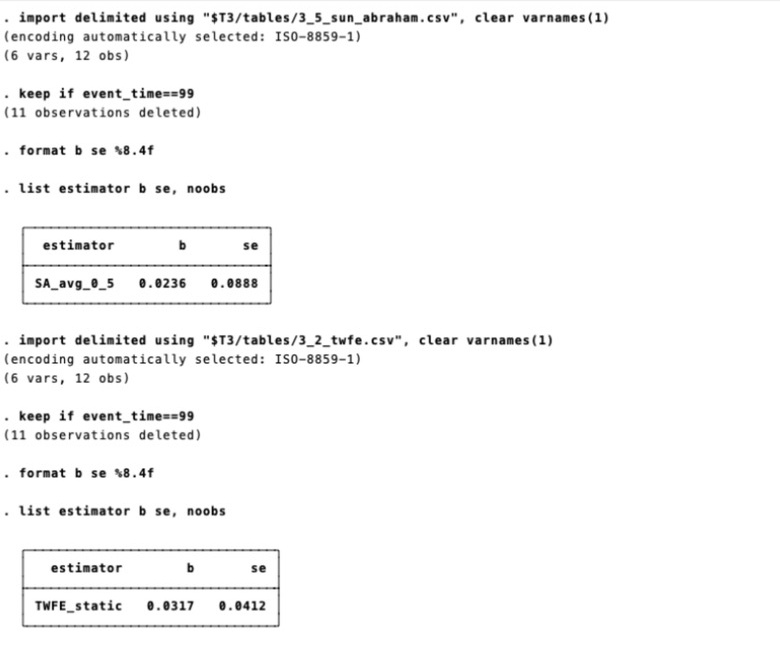
\includegraphics[width=\linewidth]{shots/c_s5b.jpg}\end{subfigure}
\end{figure}
\vspace{-6pt}
\begin{table}[H]\centering\small
\caption{Average effect after the first solar policy}
\begin{tabular}{lccc}
\toprule
Estimator & Main sample & Paper-style sample & Pre-trend test\\
\midrule
Callaway--Sant'Anna & $+0.057$ (0.143) & $-0.091$ (0.120) & $p<0.001$\\
\quad conditional on urban & $+0.057$ (0.141) & -- & \\
Borusyak--Jaravel--Spiess & $+0.078$ (0.069) & $-0.087$ (0.060) & $p=0.239$\\
Sun--Abraham (years 0--5) & $+0.024$ (0.089) & -- & \\
TWFE (static, benchmark) & $+0.032$ (0.041) & -- & $p=0.341$\\
\bottomrule
\end{tabular}
\par\smallskip\footnotesize SE in parentheses, clustered by county. None of the estimates is statistically significant.
\end{table}

\subsection*{How to read the event-study graphs}
\begin{whybox}\small
The x-axis is years relative to the first solar policy (0 = first year; $-1$ = reference). Dots are the estimated difference in bird diversity compared with similar counties, and vertical lines are 95\% confidence intervals (crossing zero means the result could be chance). \textbf{Before the policy} the dots should be near zero (parallel trends). \textbf{After the policy}, if solar policy harmed birds, the dots would fall below zero.
\end{whybox}

\subsection*{Main sample}
\begin{figure}[H]\centering
\begin{subfigure}{0.49\linewidth}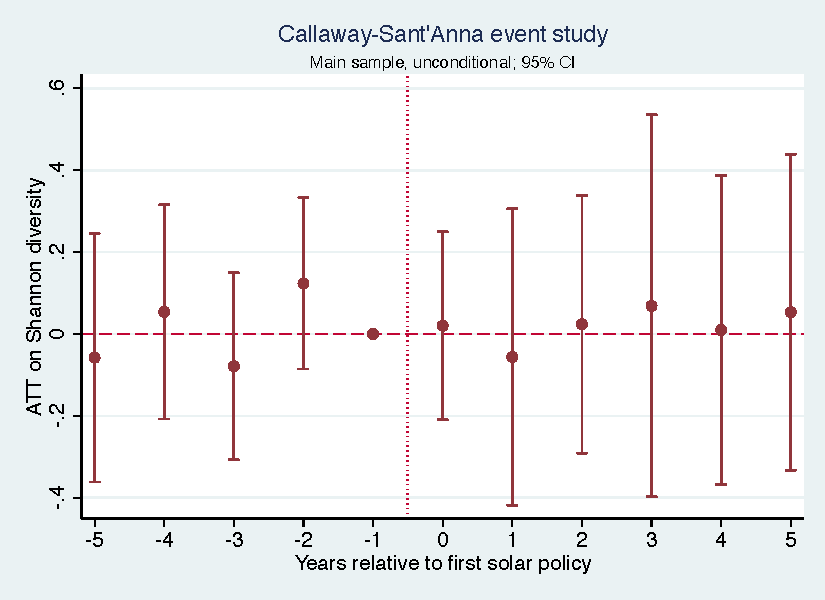
\includegraphics[width=\linewidth]{fig/3_3_event_study_cs_1.pdf}\caption{Callaway--Sant'Anna}\end{subfigure}
\begin{subfigure}{0.49\linewidth}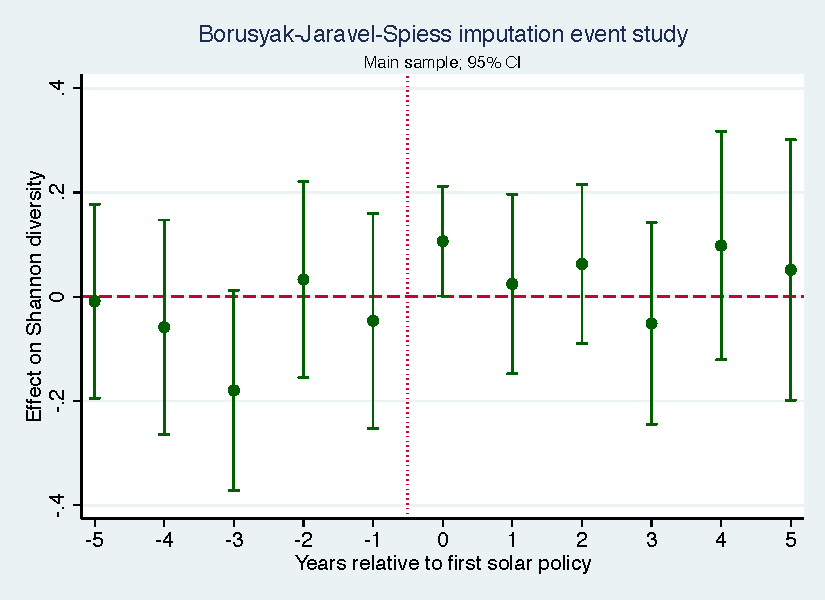
\includegraphics[width=\linewidth]{fig/3_4_event_study_bjs_1.pdf}\caption{Borusyak--Jaravel--Spiess}\end{subfigure}\\[4pt]
\begin{subfigure}{0.49\linewidth}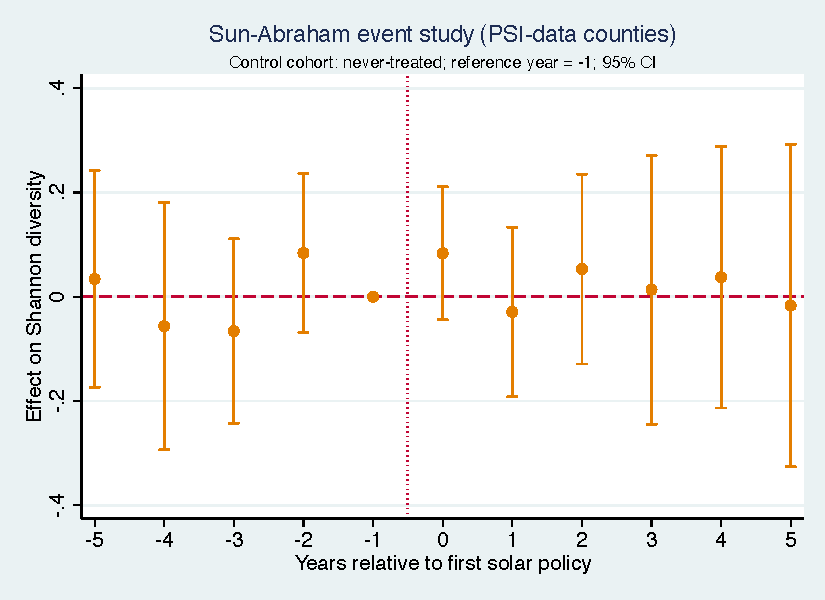
\includegraphics[width=\linewidth]{fig/3_5_event_study_sa.pdf}\caption{Sun--Abraham}\end{subfigure}
\begin{subfigure}{0.49\linewidth}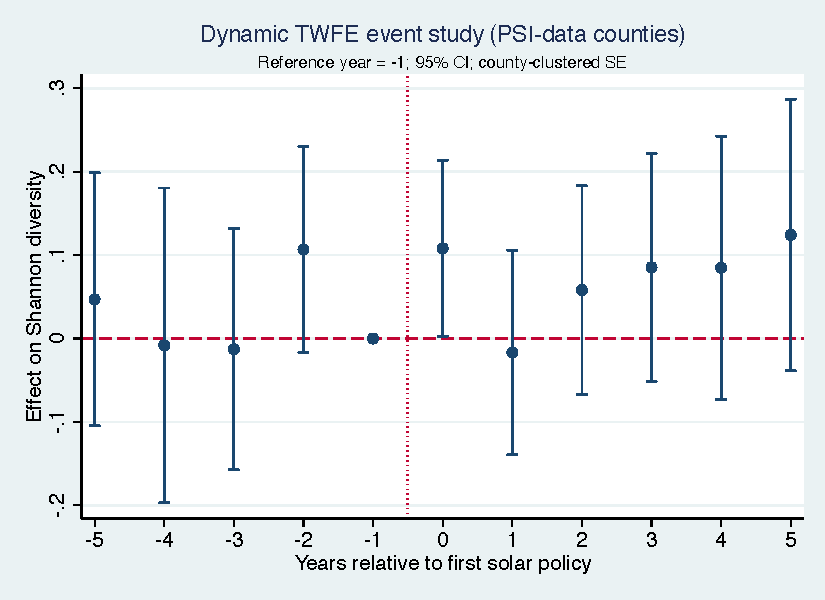
\includegraphics[width=\linewidth]{fig/3_2_event_study_twfe.pdf}\caption{Conventional TWFE event study}\end{subfigure}
\caption{Bird diversity before and after a county's first solar policy (main sample).}
\end{figure}
\begin{whybox}\small
\textbf{What these show.} After the policy (years 0--5) the dots stay around zero or slightly \emph{above} it, and almost every interval crosses zero. \textbf{There is no drop in bird diversity.} The only years clearly different from zero are year 0 in BJS and TWFE (about $+0.11$), which are increases.
\end{whybox}

\subsection*{Paper-style sample}
\begin{figure}[H]\centering
\begin{subfigure}{0.49\linewidth}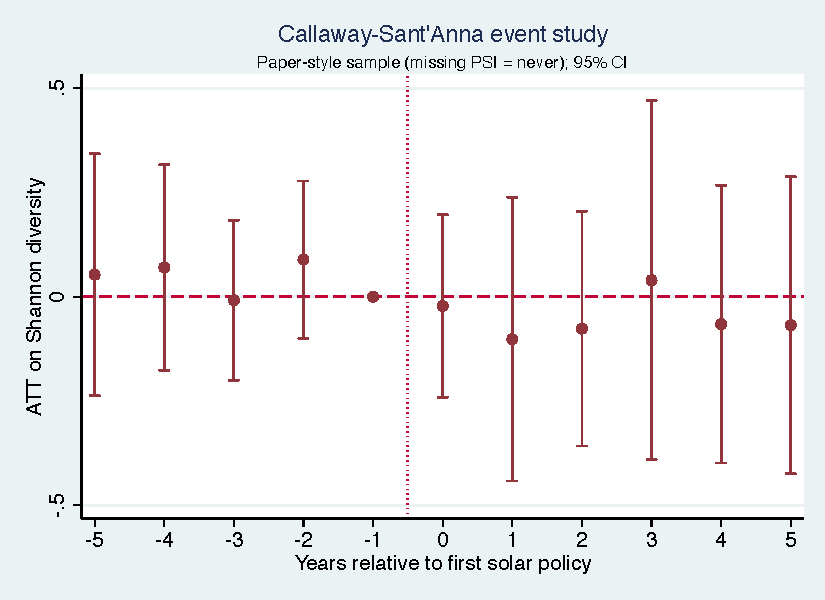
\includegraphics[width=\linewidth]{fig/3_3_event_study_cs_3.pdf}\caption{Callaway--Sant'Anna}\end{subfigure}
\begin{subfigure}{0.49\linewidth}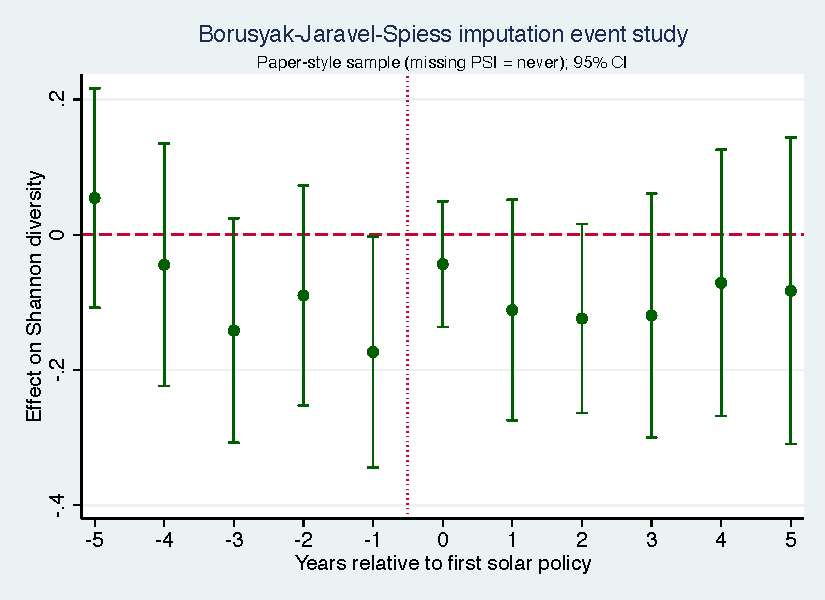
\includegraphics[width=\linewidth]{fig/3_4_event_study_bjs_2.pdf}\caption{Borusyak--Jaravel--Spiess}\end{subfigure}
\caption{The same analysis when missing-PSI cities are counted as ``never treated''.}
\end{figure}
\begin{whybox}\small
\textbf{What these show.} With the missing-data cities as controls, the post-policy dots turn negative (CS $-0.091$, BJS $-0.087$, both insignificant). But in the BJS graph the dots are \emph{already below zero before the policy}, and at $-1$ the gap is $-0.173$ (significant). These counties were already falling behind the cities before any solar policy. The negative ``effect'' is a pre-existing difference, the same city-vs-countryside problem as in Task 1.
\end{whybox}

\paragraph{Caveat.} The CS pre-trend test rejects ($p<0.001$), though the BJS ($p=0.24$) and TWFE ($p=0.34$) tests do not, and some groups are tiny (2 counties in 2020). The designs are not perfect, but \textbf{none shows harm}.

%==========================================================================
\section{Conclusion}
\begin{table}[H]\centering\small
\begin{tabularx}{\linewidth}{>{\raggedright\arraybackslash}p{3.6cm}>{\raggedright\arraybackslash}X>{\raggedright\arraybackslash}p{3.2cm}}
\toprule
Task & Finding & Supports harm?\\
\midrule
1. Reproduction & All 12 numbers match exactly & (code is correct)\\
1.1 Data & 724 mostly urban counties have missing PSI coded as 0 & --\\
1.3 TWFE fair comparison & $-0.0125 \to -0.0027$ ($p=0.47$) & No\\
1.3 IV & Fails zero-first-stage test ($p=0.048$) & Not reliable\\
1.3 PSM & Weights never applied; with weights, insignificant & No\\
2. Sensitivity & RV 2.2\%, $RV_\alpha$ about 1\%; urban trend far stronger & No, fragile\\
3. Staggered DiD & All four estimators small, positive, insignificant & No\\
\bottomrule
\end{tabularx}
\end{table}

\begin{summarybox}
\small
\textbf{What we can say:} ``The paper's results are computationally reproducible. But when we compare similar places, test for hidden factors, or follow counties before and after their first solar policy, the negative effect disappears or turns slightly positive and insignificant. So this study's data do not show that solar policy harms bird diversity. The negative result is most likely caused by comparing countryside counties with cities that have missing data.''\\[4pt]
\textbf{What we should not say:} that solar policy has \emph{no} effect on birds, or that it \emph{helps} them. Our estimates are too uncertain for either claim.
\end{summarybox}

\section*{References}
\small
\begin{itemize}[leftmargin=12pt]
\item Baker, A., Callaway, B., Cunningham, S., Goodman-Bacon, A., and Sant'Anna, P.\ H.\ C. Difference-in-differences designs: a practitioner's guide. \textit{Journal of Economic Literature} (doi 10.1257/jel.20251650).
\item Borusyak, K., Jaravel, X., and Spiess, J.\ (2024). Revisiting event-study designs. \textit{Review of Economic Studies} 91(6).
\item Callaway, B., and Sant'Anna, P.\ H.\ C.\ (2021). Difference-in-differences with multiple time periods. \textit{Journal of Econometrics} 225(2).
\item Cinelli, C., and Hazlett, C.\ (2020). Making sense of sensitivity: extending omitted variable bias. \textit{JRSS Series B} 82(1), 39--67.
\item Sun, L., and Abraham, S.\ (2021). Estimating dynamic treatment effects in event studies. \textit{Journal of Econometrics} 225(2).
\item van Kippersluis, H., and Rietveld, C.\ A.\ (2018). Beyond plausibly exogenous. \textit{Econometrics Journal} 21(3).
\item Zhang et al.\ (2026). China's solar expansion policy reduces bird diversity. \textit{Science} 393, 831.
\end{itemize}

\end{document}
